\documentclass[conference]{IEEEtran}
\usepackage[utf8]{inputenc}
\usepackage{graphicx}
\usepackage{url}
\usepackage{amsmath}
\usepackage{amsfonts}
\usepackage{amssymb}
\usepackage{ulem}

\def\NewL{\\\noindent\hspace*{5mm}}

\begin{document}
\title{HRTF Individualised Mag-LS and COMPASS Ambisonics-To-Binaural Rendering:
Overall Perceived Quality for Pre-Conditioned Listeners\\
{\footnotesize precis reviewed, open access paper for 154th
Audio Eng. Soc. Conv., Espoo, 2023
Paper xxxxx, \url{http://www.aes.org/e-lib/browse.cfm?elib=xxxxx}}}
\author{
\IEEEauthorblockN{
Frank Schultz\IEEEauthorrefmark{1},
Shaimaa Doma\IEEEauthorrefmark{2},
Sascha Spors\IEEEauthorrefmark{1},
Janina Fels\IEEEauthorrefmark{2}}
\IEEEauthorblockA{\IEEEauthorrefmark{1}Institute of Communications Engineering, University of Rostock, Germany}
\IEEEauthorblockA{\IEEEauthorrefmark{2}Institute for Hearing Technology and Acoustics, RWTH Aachen University, Germany}
}
\maketitle
\thispagestyle{plain}
\pagestyle{plain}

\section*{Abstract}
Headphone-based spatial audio reproduction nowadays often uses Ambisonics-to-binaural rendering.
%
For optimum beamforming, non-parametric methods, such as the Magnitude Least Squares (Mag-LS), and parametric methods, such as the coding and multidirectional parametrisation of Ambisonic sound scenes (COMPASS), were recently introduced.
%
The use of individual (rather than non-individual) head-related transfer functions (HRTFs) technically optimises rendering.
%
We present listening experiment results, indicating significantly higher overall perceived quality ratings of renderings with individual HRTFs than with non-individual HRTFs for a pre-conditioned participant focusing on externalisation and localisation.

\section{Introduction}
%
In the audio community, Ambisonics \cite{Zotter2019_Ambisonics} refers to sampling/encoding and reconstructing/decoding sound fields with respect to spherical geometries.
%
Presumably due to practical convenience in fabricating spherical recording microphone arrays and (semi)-spherical-like reproduction loudspeaker arrays, as well as due to highly direction-independent beamforming capabilities, Ambisonics advanced to a very important spatial audio technique.
%
Another prominent, but rather personal spatial audio approach is binaural rendering using headphones \cite{Moeller1992}, which aims at reproducing the incident signals of spatial sound scenes at human ear canal entrances.
%
This method benefits from the fact that healthy-hearing humans evaluate their HRTFs \cite{Moeller1992} (cf. highly individual, frequency-dependent, distinctive antenna directivities) of their ear pairs (cf. two-channel receiver antennas) for spatial hearing.
%
\NewL Combining both approaches \cite{McKeag1996}, i.e. using Ambisonics for sound field recording and using headphones for binaural playback, might appear meaningful, because i) we might wish to listen to headphones rather than to loudspeaker arrays in certain applications and ii) the acquisition of HRTFs and of sound field information along a spherical surface can be treated separately and thus (re)-combined variously.
%
From a signal-theoretical viewpoint, this results in a joint sampling problem \cite{BenHur2018}.
%
The inherently related reconstruction problem can be referred to as Ambisonic decoding to headphones \cite[Ch.~4.11]{Zotter2019_Ambisonics}, binaural rendering of Ambisonics signals \cite{Zaunschirm2018}, and binaural decoding \cite{Politis2016_diss}.
%
Two strategies for reconstruction, i.e., finding an appropriate beamformer, are nowadays followed: i) non-parametric methods and ii) parametric methods, cf. \cite{Politis2016_diss}.
%
They fundamentally differ in how the captured signals are treated to calculate a beamformer, and naturally, for each strategy there exist numerous solutions with pros and cons.
%
For both strategies, meanwhile real-time capable rendering plugins are available, e.g. \cite{McCormack2019}, which can load HRTFs via SOFA files.
%
\NewL Non-parametric beamformers might include psychoacoustic considerations and exhibit a linear, static decoder matrix based on the chosen HRTF set.
%
The most recent and mature non-parametric approaches are (comparatively) discussed in \cite{Zaunschirm2018, Schoerkhuber2018_MagLS, Luebeck2020, Deppisch2021, Engel2022}, \cite[Ch.~4.11]{Zotter2019_Ambisonics}.
%
These indicate that the Mag-LS family, introduced in \cite{Schoerkhuber2018_MagLS, Deppisch2021}, seems to be a robust candidate for optimum beamforming with comparatively well-tempered perceptual consequences.
%
\NewL Parametric beamformers exhibit a sound field analysis stage, typically accompanied by a psychoacoustic model, and a rendering stage.
%
Note that from a signal theory viewpoint, this is all related to the reconstruction stage, as the signals to work on are already spatio-temporally sampled.
%
Direct sound and diffuse sound are often rendered independently, requiring their time-dependent estimation and separation.
%
Hence, beamforming typically incorporates linear and time-varying decoder matrices.
%
Parametric approaches are discussed in \cite{Politis2016_diss, Politis2017_Waspaa, Politis2018_Compass, Schoerkhuber2019, McCormack2019_EAA}.
%
The COMPASS \cite{Politis2018_Compass} is a prominent parametric beamformer that uses null-steering based beamforming within the Ambisonics modal domain to separate direct and diffuse sound.
%
The same mindset is followed in \cite{Schoerkhuber2019}, yet applying other optimization constraints.
%
One inherent, potentially highly useful, feature of these beamformers is the usage of unaltered HRTF information for signal parts that are estimated as direct sound.
%
\NewL For both parametric and non-parametric beamformers, using individual HRTFs is an optimum choice in a technical sense, as it reflects the technically most precise antenna directivity compared to non-individual HRTFs.
%
However, does this technical individualisation aspect necessarily and obviously reflect highest overall perceived quality, relative to the listener's own internal reference for Ambisonics decoding to headphones?
%
To contribute to this ongoing research question---the results of \cite{Armstrong2018} indicate a preference of non-individual (especially those of the tested HATS) over individual, diffuse-field equalised HRTFs---we designed and conducted several listening tests.
%
\NewL To cover the current practical workflows of higher order Ambisonics (HOA), we are here especially interested in the HRTF individualisation while using HOA up to 7th order.
%
Further, it is typical that spatial sampling of HRTFs is much finer than that of sound fields, hence spatial resolution of the two data sets differ by roughly one order of magnitude in our considerations.
%
The implications of this sampling mismatch are meanwhile well understood in terms of signal processing and perceptual consequences, which in fact motivated many beamforming strategies mentioned above.
%
\NewL In terms of operationalisation of the research question, we shall test the hypothesis $H_0$ that overall perceived quality is equal using individual HRTFs and
non-individual HRTFs in HOA-to-binaural rendering.
%
In our studies, this is tested for HOA up to 7th order for a music and for a female-speech scene in dedicated rooms, applying %and
one parametric (COMPASS) and one non-parametric (Mag-LS) beamforming strategy.


\section{Methods}
%
The study presented here was a by-product of preparing a larger experiment, asking participants to rate overall perceived quality of HOA-to-binaural renderings incorporating individual and non-individual HRTFs.
%
Hence, firstly, we briefly summarise general issues of this experiment, which is discussed in detail in \cite{Schultz2023_Acta}.
%
Afterwards, aspects that are specific for this paper's study are stated.

\subsection{General Considerations}

Besides numerous technical details, foundational choices might have a fundamental impact on the findings.
%
We consider the aspects i) use of frontal audio scenes, i.e., the virtual sources exhibit highly frontal direct sound incidences, thus only the room reflections are fully 3D distributed, ii) 3D head-rotation tracking instead of only azimuthal tracking, iii) no visual support of the scene, and iv) musical preference might bias quality rating, being such fundamental choices.



\subsubsection{HRTF / HpTF Measurements}
Free-field HRTFs were measured for the G.R.A.S. KEMAR 45BA head and torso simulator (HATS) with large, shore 00-55 pinnae, for the Aachen HATS \cite{schmitz1995_KKac} and for all participants using a loudspeaker arc installed in a hemi-anechoic chamber. With 64 loudspeakers of 1~inch diameter at a radius of 1.2~m, the arc covers zenith angles up to 160~deg. Using two three-axis lasers, the interaural axis was set to the centre of the arc at 2~m height. The built-in microphones were used for both HATS, whereas Sennheiser KE3 microphones, fixated within closed power domes, were inserted at the human ear canal entrances and taped to the sides of the neck using medical adhesive bands.
\NewL During the measurement of ca. 5~min, the arc rotated continuously around the subject \cite{richter2019_influence} while emitting interleaved exponential sweeps \cite{majdak2007_mesm,dietrich2013_optMesm}.
Post-processing comprised deconvolution with an individual sweep, cropping and windowing the acquired impulse responses to eliminate ground reflections.
Then followed a division by reference spectra acquired in absence of the head, with regularization after \cite{kirkeby1998_reg}.
Due to the difficulty of dismantling the built-in microphones of the HATSs, a G.R.A.S. 40 AF microphone was used.
\NewL After division, low-frequency data were extrapolated towards a magnitude and phase of 0~dB/0~deg.
The HRTFs were then mapped to the corresponding time- and frequency-dependent loudspeaker positions. The resulting frequency-dependent spatial grids were interpolated to a common equiangular grid of 2.5~deg resolution and stored as SOFA files.
\NewL  The Sennheiser HD650 headphones used in the experiment were equalised for each participant and HATS. Following \cite{masiero2011_HpTF}, the headphone equalization function (HpEQ) was calculated from ten repeated headphone transfer function (HpTF) measurements.
Measurements and processing were done using the ITA-Toolbox \cite{ITA-Toolbox_2017} in MATLAB.

\subsubsection{Audio Material / Ambisonics Scenes / Binaural Rendering}
%
In the listening test, one music content and one female-speech content were employed for binaural renderings.
%
The 11~s raw music was taken from the anechoic database project \cite{Therry2019_ICA}; more specifically, the clarinet, double bass and guitar trio performance of the Bechet piece was used.
%
The 10~s anechoic speech stimulus was created from 5 short, disconnected sentences taken from an audio book\footnote{Kati Naumann, Was uns erinnern lässt, Harper Collins / Lübbe Audio, 2019, read by Ilka Teichmüller}, whose content is highly anechoic.
%
%CD/Track
%6/12 Elvira lies den Blick durch den Raum wandern.
%3/6 Willst Du die Gerda nicht mal mitbringen?
%5/18 Das Telefon klingelte.
%5/6 Das Tauwetter setzte ein.
%1/7 Der Hund drehte sich von Miller weg.
%
\NewL Two shoebox rooms with dedicated room acoustic parameters for music and speech performances were simulated with RAVEN \cite{schroder2011_raven}, yielding 7th order HOA encoded room impulse responses (RIRs) from an ideal, infinitesimal microphone array.
%
We therefore did not consider the end-to-end Mag-LS beamforming \cite{Deppisch2021}.
%
For the music stimulus, a concert hall dedicated for chamber music with
$(23\times 11\times 7)\,\mathrm{m}^3$, $\mathrm{T}_{60,\mathrm{mean}} \approx 1.3\,\mathrm{s}$, was created, setting the trio in a typical frontal stage (with a slight left offset) scenario and considering a seated listener roughly 4 m away from the clarinet, which acts as the centred solo instrument.
%
For the female speech stimulus a seminar room with $(10\times 7\times 4)\,\mathrm{m}^3$, $\mathrm{T}_{60,\mathrm{mean}} \approx 0.6\,\mathrm{s}$
was created, setting the seated speaker in a typical front-central presentation scenario and considering a standing listener almost exactly in the centre of the room, about 3.5 m away of the speaker.
%
\NewL HOA-RIRs were convolved with the anechoic audio material; in the case of the music trio, the three instrument-specific Ambisonics signals were additionally superimposed with equal levels.
%
For each audio stimulus, a 7th order/64-channel HOA signal represents the spatial scene, which we refer to as an Ambisonics scene in the following.
%
\NewL For HOA-to-binaural real-time rendering, VST plugins from the Sparta suite\footnote{\url{https://leomccormack.github.io/sparta-site/}, v1.6.2} were utilised.
%
The Sparta \textit{AmbiBin} plugin with Mag-LS and enabled phase simplification (all other options opted out) was chosen to involve a non-parametric beamforming strategy.
%
The COMPASS \textit{Binaural} plugin with MUSIC as DoA estimator and ambient mode KT-CM for speech and KT-MWF for music (all other settings as default) was chosen as a parametric beamforming strategy.
%
HpEQs were handled as FIR filters by the Sparta \textit{MultiConv} plugin.

\subsubsection{Hard- and Software Tools}
%
A 2021 MacBook Pro (M1 Pro, 32GB RAM) and a RME Fireface UC soundcard were used for execution of the listening tests with Rec. ITU BS.1170 calibrated, constant playback level for all stimuli.
%
The graphical user interface (GUI), cf.~Fig.~\ref{fig:gui}, is hosted in a Jupyter notebook with GUI elements realised as Jupyter widgets\footnote{\url{https://ipywidgets.readthedocs.io}}.
%
\begin{figure}[t!]
\centering
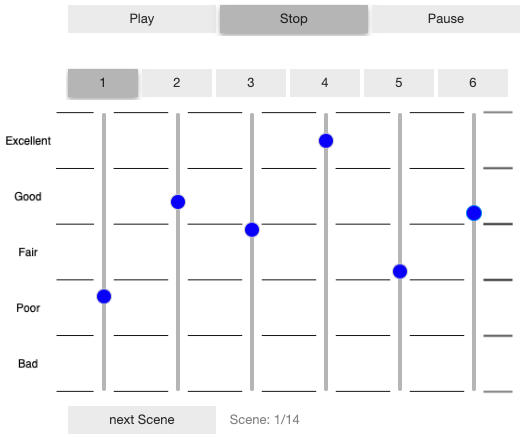
\includegraphics[width=0.495\textwidth]{../graphics/GUI.png}
\caption{GUI for the listening test running within a Jupyter notebook using Jupyter widgets. Quality scale according to Rec. ITU-R BS.1534-1.}
\label{fig:gui}
\end{figure}
%
Reaper, as VST host and DAW, served as real-time rendering and playback software for the binaural audio stimuli.
%
The GUI remotely controlled Reaper via reapy package\footnote{\url{https://python-reapy.readthedocs.io/}}.
%
This handling was used to load projects, control playback, bypass FX etc.
%
The VST plugin ABComparison\footnote{\url{https://github.com/DanielRudrich/ABComparisonPlugin}, v1.4.0} was used for binaural stimuli switching with cross-fading, controlled by the GUI via OSC commands using python-osc\footnote{\url{https://pypi.org/project/python-osc/}}.
%
3D head rotations were tracked with a Supperware Ltd's Head Tracker 1 mounted onto the HD650.
%
Supperware's Bridgehead app communicated with the Sparta \textit{Rotator} plugin via OSC.
%
Dynamic binaural synthesis is thus realised by 3D rotating the Ambisonics scene ahead of the actual binaural decoding.

\subsubsection{Listening Test Design}
%
In order to set up 14 dedicated rating panels, rendering approaches (Sparta and COMPASS), HOA orders (1st, 2nd, 3rd; for Mag-LS also 7th) and the two above-mentioned Ambisonics scenes (speech in seminar room, trio in concert hall) were interchangeably combined.
%
For each panel, spatial-audio-experienced participants were asked to rate the overall perceived quality of six binaural playbacks relative to their own internal reference, cf.~Fig.~\ref{fig:gui}.
%
These were rendered using different HRTF sets:
%
\begin{itemize}
\item[1.] own individual HRTFs, with maximum available HOA order, i.e. 7th for Sparta and 3rd for COMPASS (\texttt{own max})
\item[2.] own individual HRTFs (\texttt{own})
\item[3.] HRTFs from KEMAR HATS (\texttt{kem})
\item[4.] HRTFs from Aachen HATS (\texttt{ac})
\item[5.] random human HRTFs \#1, randomly chosen for each panel and each participant, excluding their own and those from 6. (\texttt{r1})
\item[6.] random human HRTFs \#2, randomly chosen for each panel and each participant, excluding their own and those from 5. (\texttt{r2})
\end{itemize}
using a dedicated HOA order for HRTF options 2.--6., and either Sparta or COMPASS, and either music or speech Ambisonics scene.
%
Each participant thus was asked to rate overall perceived quality for
2 audio $\times$ 4 HOA order $\times$ 6 HRTF = 48 items for Sparta-based renderings and 2 audio $\times$ 3 HOA order $\times$ 6 HRTF = 36 items for COMPASS-based renderings, in total 84 items allotted to 14 panels, cf.~Fig.~\ref{fig:boxplot_sparta} and \ref{fig:boxplot_compass}.
%
\NewL Note that no anchor and no known and/or hidden reference is intentionally given in the panels.
%
Hence, we do not refer to the listening test as MUSHRA or as MUSHRA-like.
%
The chosen test design rather covers the practical aspect of selecting perceptually appropriate HRTFs out of several available options.
%
If the considered HOA-to-binaural rendering using individual HRTFs technically would outperform by orders of magnitude, one could assume that this would be a self-evident choice, i.e., it yields by far the highest overall perceived quality.
%
Our chosen test design shall explicitly check, if this is the case or rather not (which actually is not possible with a MUSHRA design).
%
Note that the HRTF option \texttt{own max} might be interpreted as a reference-like stimulus, as it is the signal with highest technical quality per panel.
%
However, we intentionally included this option to check if HOA order dependencies can be observed within and over the panels, rather than providing this as a reference with all the expectations being implied on the reference stimulus by a true MUSHRA test.
%
\NewL For the study \cite{Schultz2023_Acta}, twelve participants were asked to rate the 14 panels on perceived overall quality.
%
Participants were informed that dynamic binaural reproduction with head rotation tracking was utilised, asking to use this feature for evaluation.
%
Further, it was communicated to them that at least one of the six renderings per panel used their own HRTFs.
%
No other information about the rendering technique was given, so especially, it was not known that HOA-to-binaural rendering is involved.
%
Before the actual test, a training allowed for comparing with the internal reference.
%
For that, music and speech scenes were rendered with own HRTFs and highest available HOA order.
%
The ratings of this study indicate that renderings with own HRTFs do not obviously and not necessarily yield highest overall perceived quality ratings.
%
This might be explained by individually different quality concepts and by the test design without reference and anchor.


\subsection{Specific Considerations for Preconditioning}
%
For the experiment presented here, the same listening test environment and test design as described above, was used.
%
It however includes only one pre-conditioned participant, who was naturally not part of the above summarised study \cite{Schultz2023_Acta}.
%
In fact, the here presented experiment was a by-product of designing and pre-testing by the main author, which we find worth sharing.
%
\NewL Obviously, the participant is considerably biased towards some aspects of the test.
%
This pre-conditioning covers:
%
First, the participant had a very pronounced expectation for highest externalisation and localisation quality, as the test introduced a very first-time experience of own HRTFs (note that participants of the blind study could have had a similar expectation due to awareness of utilising their own HRTFs).
%
Second, although the 14 panels as well as their stimuli appeared in randomised order, the participant knew about the HOA-to-binaural rendering and its occurring variations, which might raise dedicated expectations and/or assumptions while listening.
%
Third, although the six renderings per panel appeared in randomised order, the participant knew about the layout of the above described options, i.e., the HRTF variations, which again might raise dedicated expectations and/or assumptions while listening and thus potentially biased ratings.
%
\NewL The participant provided 6 test repetitions x 6 renderings x 14 scenes = 504 quality ratings, very consistently over the six repetitions.
%
The participant reported that overall perceived quality was assessed with the following order of importance: externalisation, localisation, timbre, room impression, finally followed by all remaining aspects.
%
The test was conducted in two acoustically treated, dimmed rooms over a two-week time span, using exactly the same hardware setup and software settings.
%
Note that the same two non-individual HRTF sets were used for random HRTF options \texttt{r1} and \texttt{r2}, which allows the grouping of test repetitions.
%
\NewL A statistical evaluation in the mindset of frequentist inference was performed for multiple comparisons among dependent groups with \verb|rmmcppb()| \cite[cf. Ch.~8.3.3]{Wilcox2022}, available in the packages Hypothesize for Python and WRS for R.
%
This method uses a percentile bootstrap method (20\% trimmed means, significance level $\alpha = 0.05$ for each \sout{group comparison} \underline{panel} (correction: 2023-04-29)).
%
We used \verb|rmmcppb()| with default settings as of version 1.1.0 from the Python library \textit{Hypothesize}~\cite{Campopiano2020_Hypothesize}\footnote{\url{https://alcampopiano.github.io/hypothesize/}}.
%
Note that the results should be handled with care, as all data originate from the very same person and thus the ratings within a single group are also dependent in the strict sense.

\section{Results}
%
Raw data of the ratings and the proposed statistical evaluation with Python is freely available\footnote{\url{https://github.com/spatialaudio/paper-aes154-individual-hrtf-hoa2binaural}}.
%
All ratings can be conveniently depicted as boxplots in the Fig.~\ref{fig:boxplot_sparta} for Sparta renderings and in the Fig.~\ref{fig:boxplot_compass} for COMPASS renderings.
%
The 14 panels (represented by 14 coloured rectangular patches) are meaningfully arranged over four plots in the two figures.
%
Each panel is comprised of six renderings, varying the independent variable \textit{HRTF}.
%
A specific boxplot slice evolves from the six repetition ratings for the dependent variable \textit{overall perceived quality} of a specific rendering.
%
\begin{figure*}[t]
\begin{center}
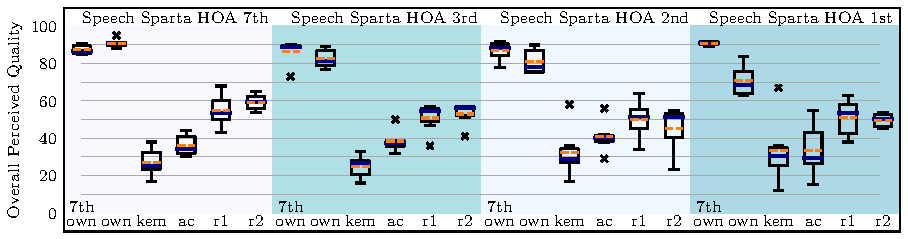
\includegraphics[width=1\textwidth]{../graphics/speech_sparta_aes154.pdf}
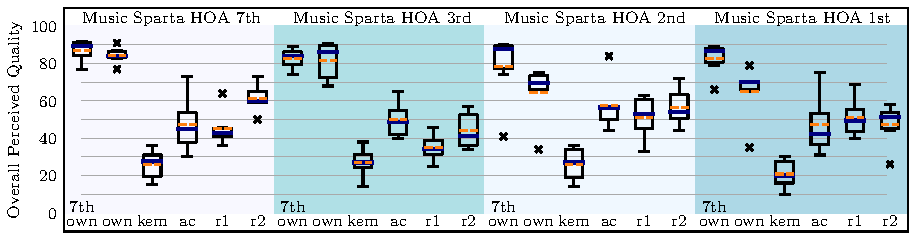
\includegraphics[width=1\textwidth]{../graphics/music_sparta_aes154.pdf}
\caption{Results as boxplots (median: blue, mean: dashed orange, interquartile range (IQR), 1.5-IQR for whiskers, outliers as $\times$) for speech scene (top) and music scene (bottom) rendered with Sparta plugin, i.e. Mag-LS algorithm. HRTF: \texttt{own} individual, \texttt{kem} KEMAR HATS, \texttt{ac} Aachen HATS, \texttt{r1/r2}: random human.}
\label{fig:boxplot_sparta}
\end{center}
\end{figure*}
%
\begin{figure*}[h!]
\begin{center}
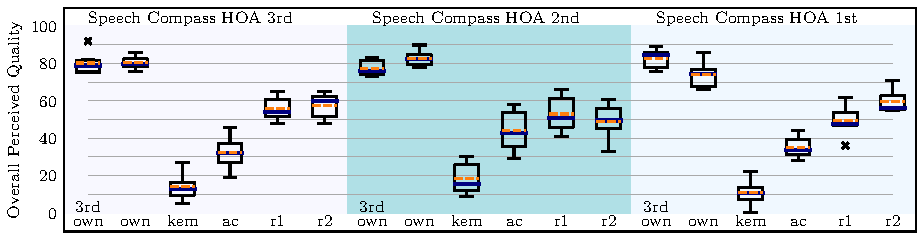
\includegraphics[width=1\textwidth]{../graphics/speech_compass_aes154.pdf}
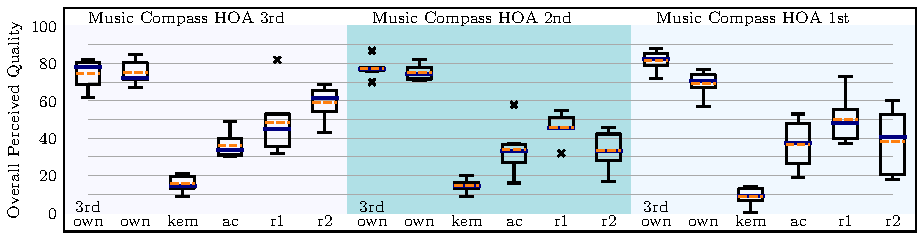
\includegraphics[width=1\textwidth]{../graphics/music_compass_aes154.pdf}
\caption{Results as boxplots for speech scene (top) and music scene (bottom) rendered with COMPASS plugin. Same depiction strategy as in Fig.~\ref{fig:boxplot_sparta} above.}
\label{fig:boxplot_compass}
\end{center}
\end{figure*}
%
\NewL To substantiate some apparent boxplot-driven indications, hypothesis tests for mean differences of two groups can be performed with the above-mentioned bootstrap approach.
%
For each panel 15 group comparisons (\texttt{r2} vs. \texttt{r1}, \texttt{r2} vs. \texttt{ac}, \texttt{r2} vs. \texttt{kem} ...) are possible.
%
Hence, in total $(2 \times 4 + 2 \times 3) \cdot 15 = 210$ group comparisons can be performed.
%
As the bootstrap sampling is meaningfully to be used with a random seed, results may slightly vary over multiple evaluations.
%
With the exception of three borderline group pairs, where significance varies over different statistical evaluations, all other results indicate unambiguous $p$-values (either very large or small compared to the critical $p$-value) to account for the hypothesis test.
%
\NewL We should not reject H$_0$ (i.e., considering that the group means are equal) for 59 (including the three borderline cases) out of the 210 pair-wise tests. Details can be found in the published Jupyter notebook.
% \begin{itemize}
% \setlength\itemsep{-0.25em}
% \item Speech Sparta 7th: own 7th vs. own, r1 vs. r2, kem vs. ac (borderline candidate)
% \item Speech Sparta 3rd: own 7th vs. own, r1 vs. r2
% \item Speech Sparta 2nd: own 7th vs. own, kem vs. ac, kem vs. r1, kem vs. r2, ac vs. r1, ac vs. r2, r1 vs. r2
% \item Speech Sparta 1st: kem vs. ac, kem vs. r1, kem vs. r2, ac vs. r2, r1 vs. r2
% \item Music Sparta 7th: own 7th vs. own, ac vs. r1, ac vs. r2, r1 vs. r2 (borderline candidate)
% \item Music Sparta 3rd: own 7th vs. own, kem vs. r1, ac vs. r2, r1 vs. r2
% \item Music Sparta 2nd: own 7th vs. own, own 7th vs. ac, own 7th vs. r1, own 7th vs. r2, own vs. ac, own vs. r1, own vs. r2, ac vs. r1, ac vs. r2, r1 vs. r2
% \item Music Sparta 1st: own 7th vs. ac (borderline candiate), own vs. ac, own vs. r1, own vs. r2, ac vs. r1, ac vs. r2, r1 vs. r2
% \item Speech Compass 3rd: own 3rd vs. own, r1 vs. r2
% \item Speech Compass 2nd: own 3rd vs. own, ac vs. r1, ac vs. r2, r1 vs. r2
% \item Speech Compass 1st: -
% \item Music Compass 3rd: own 3rd vs. own, own 3rd vs. r1, own 3rd vs. r2, own vs. r1, ac vs. r1, r1 vs. r2
% \item Music Compass 2nd: own 3rd vs. own, ac vs. r1, ac vs. r2
% \item Music Compass 1st: ac vs. r2, r1 vs. r2
% \end{itemize}
%
For the remaining 151 pair-wise tests, the calculated probability \textit{of rejecting $H_0$ given that it is actually true} is well below the chosen type-I error level.
%
It is thus highly unlikely that the acquired ratings of the two groups originate from same distribution, which is typically interpreted as significant differences of group means.
%
The obtained significance checks are highly reasonable compared to visual inspection of the boxplot data.
%
\NewL It is worth to mention explicitly that all group means are significantly different for the panel ``Speech COMPASS HOA 1st'', which supports the visual impression of its boxplots very well, i.e., the top-right panel in Fig.~\ref{fig:boxplot_compass}.
%
In the following, we are exclusively interested in the pair-wise tests that include individual HRTFs, i.e. including options \texttt{own max} and/or \texttt{own}.
%
For that, significant mean differences (w.r.t. \texttt{own max}/\texttt{own} vs. other HRTFs as well as \texttt{own max} vs. \texttt{own}) are also indicated for panels \quad ``Speech Sparta 1'' \quad and \quad ``Music COMPASS 1''.
%
These results suggest that own HRTFs are a preferred choice in terms of overall perceived quality, and it also indicates, that a higher Ambisonics order is preferred compared to 1st order when using own HRTFs.
%
\NewL Non-significant results, i.e., an indication that equal means are more likely than different means, are observed when comparing \texttt{own max} vs. \texttt{own} for the panels
%
\quad``Speech Sparta 2, 3 \& 7'' \quad and
\quad``Speech COMPASS 2 \& 3'' \quad and
\quad``Music Sparta 3 \& 7'' \quad and
\quad``Music COMPASS 2''.
%
These results suggest that own HRTFs are a preferred choice against non-individual HRTFs.
%
They do not suggest, that, when using individual HRTFs, increased Ambisonics order increases quality rating.
%
\NewL The panels \quad ``Music Sparta 1 \& 2'' \quad indicate that quality rating for own HRTFs is comparably heterogeneous, because these exhibit very large outlier ranges.
%
It is thus not surprising, that bootstrapping and hypothesis testing yields a high amount of non-significant results, which in turn suggests that quality ratings do not differ considerably for \texttt{own max} vs. \texttt{own}.
%
For the panel \quad ``Music Compass 3'' \quad, non-significant results are obtained for \texttt{own max} vs. \texttt{own}, and \texttt{own max} vs. \texttt{r1}, and \texttt{own} vs. \texttt{r1} and \texttt{own max} vs. \texttt{r2}.
%
% \begin{itemize}
% \setlength\itemsep{-0.25em}
% \item Speech Sparta 7th: own 7th vs. own
% \item Speech Sparta 3rd: own 7th vs. own
% \item Speech Sparta 2nd: own 7th vs. own
% \item Speech Sparta 1st: -
% \item Music Sparta 7th: own 7th vs. own
% \item Music Sparta 3rd: own 7th vs. own
% \item Music Sparta 2nd: own 7th vs. own, own 7th vs. ac, own 7th vs. r1, own 7th vs. r2, own vs. ac, own vs. r1, own vs. r2
% \item Music Sparta 1st: own 7th vs. ac (borderline candidate), own vs. ac, own vs. r1, own vs. r2
% \item Speech Compass 3rd: own 3rd vs. own
% \item Speech Compass 2nd: own 3rd vs. own
% \item Speech Compass 1st: -
% \item Music Compass 3rd: own 3rd vs. own, own 3rd vs. r1, own 3rd vs. r2, own vs. r1
% \item Music Compass 2nd: own 3rd vs. own
% \item Music Compass 1st: -
% \end{itemize}
%


\section{Discussion}
%
The panels using Sparta HOA 7th order and COMPASS HOA 3rd order---leftmost in Fig.~\ref{fig:boxplot_sparta} and \ref{fig:boxplot_compass}---contain two exactly identical binaural renderings for the options \texttt{own max} and \texttt{own}.
%
Their boxplots with comparably small interquartile ranges (IQRs) and the non-significant results for these group mean comparisons indicate that the test person holds a highly consistent quality concept and is reliably able to recognise technically identical stimuli.
%
Note, that the above-mentioned pre-conditioning and bias might have enhanced this skill, however, we also observed such performances in the full blind study.
%
We should not overrate this observation, though, as the panels for COMPASS HOA 2nd---middle column in Fig.~\ref{fig:boxplot_compass}---exhibit about the same quality ratings (non-significant) when comparing \texttt{own max} and \texttt{own} but with different HOA order.
%
Here, it is presumably not easy to further differentiate the two stimuli in terms of perceived quality.
%
\NewL The statistical tests indicate that both individual HRTF conditions yield significantly higher quality ratings than non-individual HRTFs for all panels, except for \quad ``Music Sparta 1 \& 2'' \quad and \quad ``Music COMPASS 3''.
%
The participant reported that for speech scenes, cues for externalisation, localisation and timbre were a lot more easily accessible than for music, which supports these findings.
%
Significantly different quality ratings for individual HRTFs but different HOA orders could be observed in the panels \quad ``Speech Sparta 1'' \quad and \quad ``Speech Compass 1'' \quad  and \quad ``Music Compass 1''.
%
This indicates that not only do individual HRTFs increase quality ratings, but also an increased HOA order yields increased quality.
%
However, with our data, we can only deduce this for 1st vs. 7th order (Sparta / Mag-LS) and 1st vs. 3rd order (COMPASS), i.e., rather high difference w.r.t. spatial resolution.


\section{Conclusion}
In a listening experiment, we found higher ratings for overall perceived quality when realizing HOA-to-binaural rendering with individual HRTFs than with non-individual HRTFs for one pre-conditioned participant with special focus on externalisation and localisation, using a no anchor/no reference design.
%
Naturally these findings should not be extrapolated towards larger populations.
%
However, we are confident that non-biased, population-aimed listening tests with differentiation to externalisation, localisation and timbre, rather than our initial overall perceived quality choice, might reveal the need for HRTF-individualised HOA-to-binaural renderings for certain applications.

\bibliographystyle{IEEEtran}
\bibliography{lit}
%
\end{document}
